\section{Appendix}
\subsection{Model Evaluation Metrics}
\subsection*{Precision and Recall}
\begin{itemize}
	\item Precision: \% of selected items that are correct
	\item Recall: \% of correct items that are selected
\end{itemize}
\begin{figure}[ht]
	\centering
	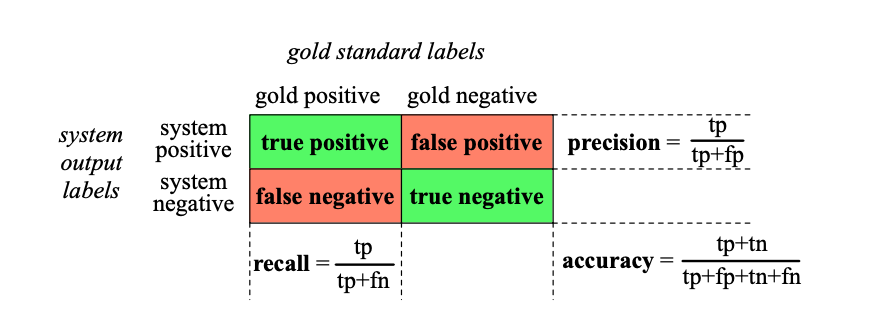
\includegraphics[width=0.7\textwidth]{figures/prec_rec.png}
	\caption{Precision and Recall}
	\label{fig:prec_rec}
\end{figure}

\subsection*{F-Measure}
\begin{itemize}
	\item Also called \textit{F-Score} $$ \mathrm{F}_\beta = \dfrac{(\beta^2 + 1) \mathrm{PR}}{\beta^2 \mathrm{P} + \mathrm{R}} $$
	\item $\beta$ controlls importance of recall and precision (typically $\beta = 1$)
\end{itemize}
